\documentclass[a4paper,oneside,reqno]{amsart}
\usepackage{pdfpages} % to include cover sheet

\input{../../../../cambridge-macros.tex}

%    Set assignment information here
\newcommand{\authorname}{Feynman Liang}
\newcommand{\coursename}{MLSALT5: Speech and Language Processing Applications}
\newcommand{\assignmentname}{Practical: Automatic MT Evaluation}

\begin{document}

%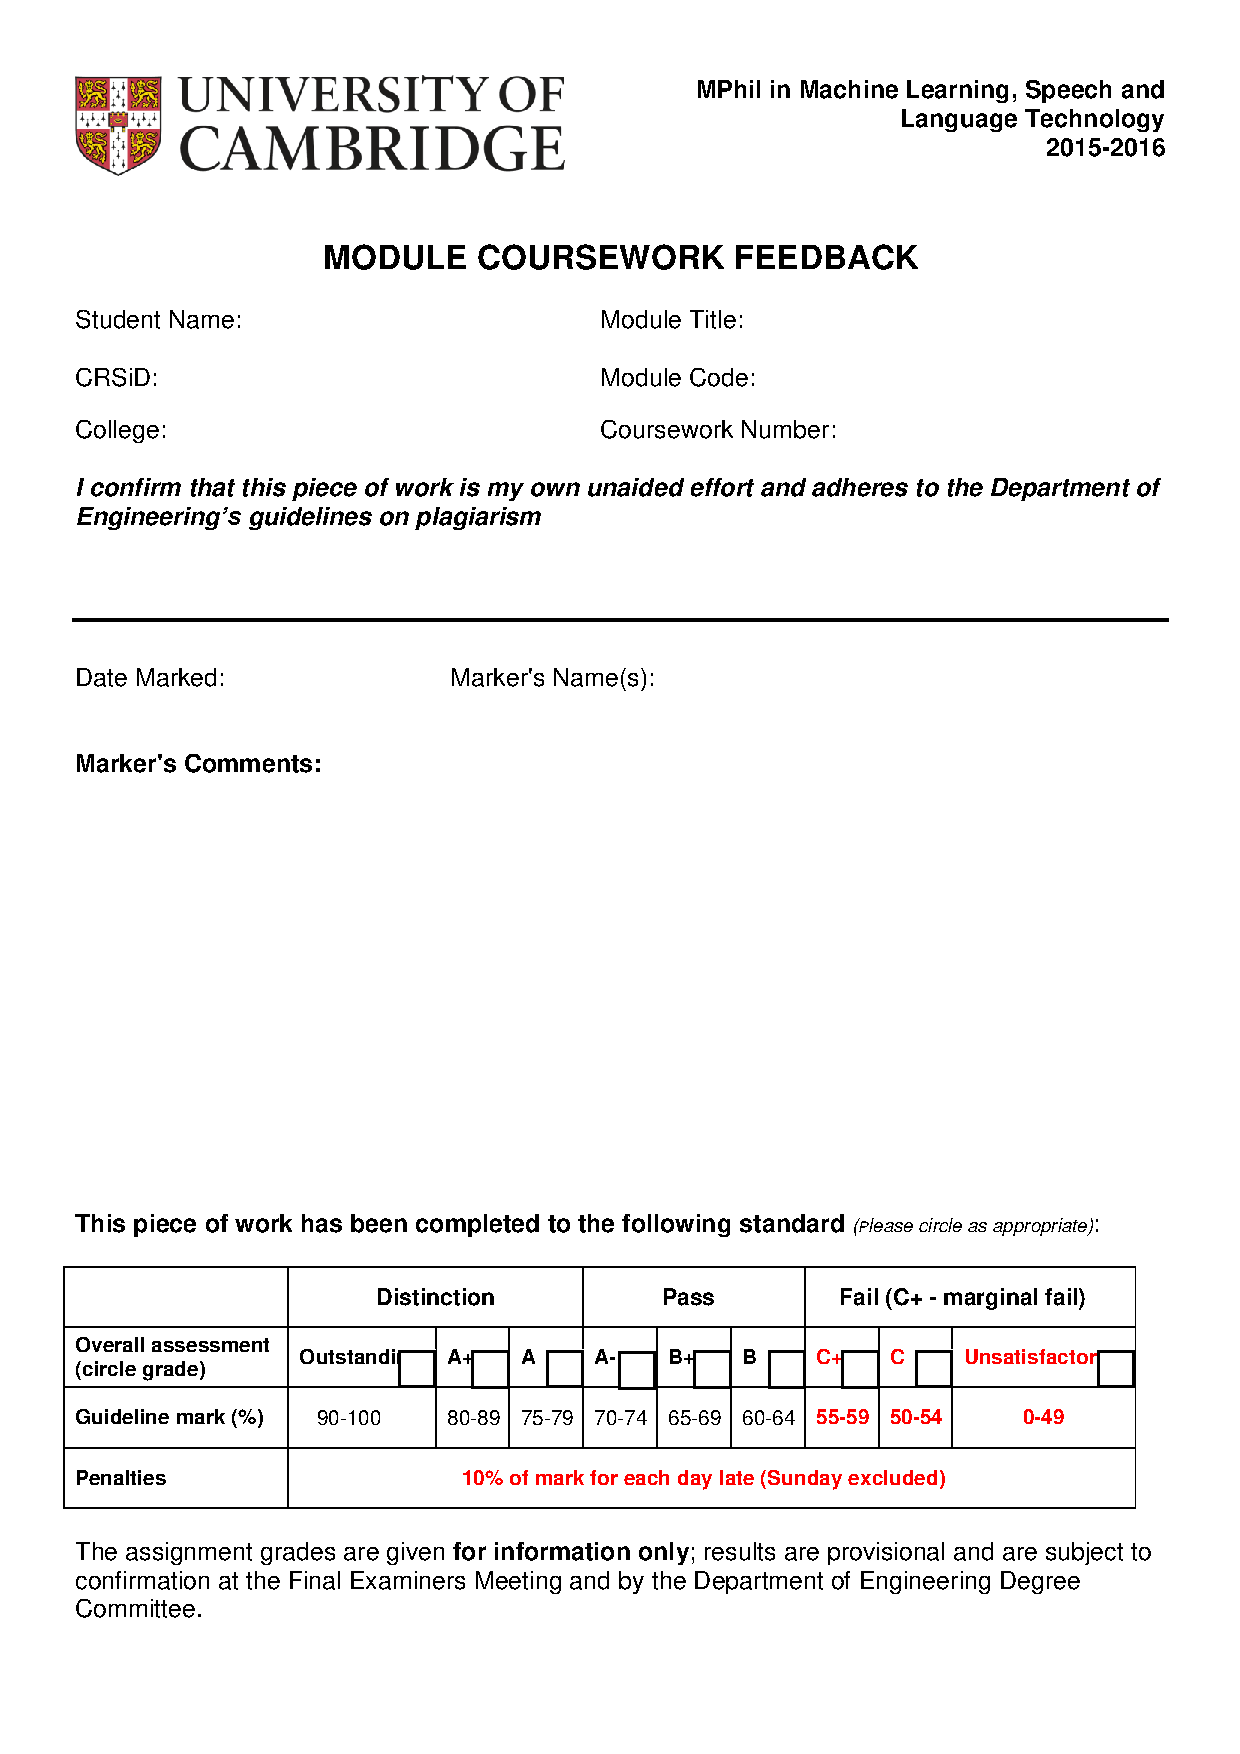
\includepdf[noautoscale]{MLSALT_Coversheet_editable.pdf}

\title{\coursename\\\assignmentname}

\author{\authorname}
\date{\today}

\maketitle

\section{New Data}

\begin{table}[ht!]
  \begin{tabular}{clcc}
    \toprule
    System                     &     & Baseline & STO \\
    \midrule
    \multirow{3}{*}{Word}      & IV  & 0.501 & 0.579\\
                               & OOV & 0.000 & 0.000\\
                               & All & 0.309 & 0.460\\
                               \hline
    \multirow{3}{*}{Word Sys2} & IV  & 0.507 & 0.585\\
                               & OOV & 0.000 & 0.000\\
                               & All & 0.403 & 0.465\\
                               \hline
    \multirow{3}{*}{Morph}     & IV  & 0.430 & 0.556\\
                               & OOV & 0.089 & 0.367\\
                               & All & 0.360 & 0.520\\
    \bottomrule
  \end{tabular}
  \caption{}
  \label{tab:}
\end{table}

\begin{table}[ht!]
  \begin{tabular}{clc}
    \toprule
    Methodology & & ATWV \\
    \midrule
    \multirow{3}{*}{CombSUM.IBM}         & IV  & 0.493 \\
                                         & OOV & 0.086 \\
                                         & All & 0.410 \\
    \multirow{3}{*}{STO-CombSUM.IBM}     & IV  & 0.601 \\
                                         & OOV & 0.366 \\
                                         & All & 0.553 \\
    \multirow{3}{*}{CombSUM.IBM-STO}     & IV  & 0.590 \\
                                         & OOV & 0.369 \\
                                         & All & 0.545 \\
    \multirow{3}{*}{STO-CombSUM.IBM-STO} & IV  & 0.601 \\
                                         & OOV & 0.364 \\
                                         & All & 0.552 \\

    \multirow{3}{*}{STO-CombSUM.All-STO} & IV  & 0.596 \\
                                         & OOV & 0.366 \\
                                         & All & 0.549 \\
    \bottomrule
  \end{tabular}
  \caption{}
  \label{tab:}
\end{table}

\begin{table}[ht!]
  \begin{tabular}{clccccc}
    \toprule
    Query Length & \# terms & Baseline & STO & CombSUM.IBM & STO-CombSUM.IBM-STO \\ % TODO: \% corpus instead of num terms
    \midrule
    1 & 28  & 0.075 & 0.360 & 0.204 & 0.443 \\
    2 & 215 & 0.433 & 0.550 & 0.440 & 0.570 \\
    3 & 100 & 0.345 & 0.554 & 0.437 & 0.575 \\
    4 & 104 & 0.369 & 0.543 & 0.436 & 0.583 \\
    5 & 30  & 0.220 & 0.384 & 0.286 & 0.413 \\
    6 & 10  & 0.094 & 0.197 & 0.197 & 0.397 \\
    7 & 1   & 0.000 & 0.000 & 0.000 & 0.000 \\
    \bottomrule
  \end{tabular}
  \caption{}
  \label{tab:}
\end{table}

% TODO: combine own systems with IBM systems

\section{1-best keyword spotting}

\subsection{Word based KWS}

\subsubsection{Implementation description}\label{sec:word-kws-impl}

We implement a word-based KWS system in the \texttt{KWSIndex} class
(\autoref{lst:kwsIndex}).  Our KWS system is constructed in the
\texttt{KWSIndex\#apply} method, which takes a CTM file, reads each line, and
parses it into a \texttt{CTMEntry} (\autoref{lst:ctmEntry}).  Each
\texttt{CTMEntry} contains the same information present in a line in a CTM file
(e.g.\ kw file, start time, duration, token). In addition, we add some
additional information such as the previous token and end times (if applicable)
to each \texttt{CTMEntry} during parsing in order to allow us to identify
\texttt{CTMEntry}s which are consecutive within the 1-best output.

These \texttt{CTMEntry}s are then added to an inverted index for quick lookup
by token. We represent the inverted index using a hashmap which is keyed on the
entry's token.  We chose to use a hashmap because it provides insertions,
updates, deletions, and lookups all in $O(1)$ amortized time and has amortized
space complexity $O(N)$ where $N$ is the number of entries.

At query time, the \texttt{KWSIndex.kws} method is called with a path
to \texttt{queries.xml}. Each query string is passed to \texttt{KWSIndex.get},
where it is split on whitespaces to yield a sequence of individual words (i.e.\ tokens),
and each token is looked up in the inverted index. This yields a sequence of collections
of \texttt{CTMEntry}s, each collection of \texttt{CTMEntry}s representing the possible
hits for that position in the query string.

We can view this as a lattice where the time axis is the position within the
query string and the collection of hits at each position nodes. Since the hits
for a query sequence should be consecutive in time, we need to find paths
through the lattice such that each node within the path appears consecutively
within the CTM file. This is where the \texttt{prevToken} and
\texttt{prevEndTime} fields of the \texttt{CTMEntry} class come in. Using this
information, we can filter all possible paths through this lattice to just
those whose sequences of \texttt{CTMEntry}s appear consecutively within the CTM
file. During this construction of paths, we also enforce the 0.5 second rule (i.e.\
the end time of each word in a path must be withn $0.5$ seconds of the next word's
start time). For each path, we set the score to be equal to the average of all the
CTM entry scores in the path because this yielded identical performance to
the reference results provided in
\path{/usr/local/teach/MLSALT5/Practical/scoring}.

After finding all valid paths, we are left with a collection of hits for the
query sequence. These hits are used to instantiate a \texttt{QueryResults}
class, whose \texttt{QueryResults.toXML} method is used to write the results in
the required KWS output format.

\subsubsection{Results for word-based KWS}

We ran our word-based KWS system on \texttt{reference.ctm} and \texttt{decode.ctm}
and ensured that our resuts (\autoref{tab:word}) matched the provided results in
\path{/usr/local/teach/MLSALT5/Practical/scoring}.

\begin{table}[ht!]
  \begin{tabular}{cccc}
    \toprule
    System                        & IV    & OOV   & All \\
    \midrule
    Word (\texttt{reference.ctm}) & 1.000 & 1.000 & 1.000 \\
    Word (\texttt{decode.ctm})    & 0.402 & 0.000 & 0.320 \\
    \bottomrule
  \end{tabular}
  \caption{TWV for word-based KWS on 1-best reference}
  \label{tab:word}
\end{table}

\autoref{tab:word} shows that our KWS system achieves 1.0 TWV on
\texttt{reference.ctm}.  This is expected because we built the KWS index on the
same reference we scored against.

When we run the system on the 1-best decoding output of a word-based ASR system
(\texttt{decode.ctm}), we obtain significantly worse results. These errors are
due to errors from the ASR system causing incorrect hits to be added to the KWS
index as well as other entries to be omitted, resulting in worse performance.
Also, notice that our out-of-vocabulary performance is $0.000$, meaning that we
were not able to find any hits for any out of vocabulary words. Since a word
based system is keyed on words in its vocabulary, any OOV words will result in
a miss. Hence, this $0.000$ TWV on OOV words is expected not only for this
system, but for any word-based KWS system.


\subsection{Morphological Decomposition}

The motivation for using morph decomposition is to better handle OOV queries.
Although a particular query word may not be in the vocabulary, by decomposing
both the query as well as the keys in the KWS inverted index into morphs, there
is a chance that the decomposed query's morphs will match with some decomposed
entry's morphs and produce a hit.

\subsubsection{Implementation details}

The \texttt{MorphDecompose} class (\autoref{lst:morphDecompose}) takes a morph
dictionary for both the CTM entries (\texttt{morph.dct}) as well as the queries
(\texttt{morph.kwslist.dct}) and provides the methods
\texttt{MorphDecompose.decomposeQuery} and
\texttt{MorphDecompose.decomposeEntry} for decomposing query sequences and
\texttt{CTMEntry}s respectively into their corresponding morph sequences. When
decomposing \texttt{CTMEntry}s, we break up each entry into multiple
entries corresponding to the individual morphs. We split the duration of a word
equally amongst its corresponding morphs. We chose score of each morph entry to be equal
to the score of the original entry so that the score assigned to a hit sequence (see
\autoref{sec:kws-word-impl}) remains the same before and after morph
decomposition. In addition, we update the \texttt{prevToken} and
\texttt{prevEndTime} fields to correctly reflect the decomposition of the
previous consecutive entry (if applicable).

The \texttt{KWSIndexMorph} class (\autoref{lst:kwsIndexMorph}) uses
\texttt{MorphDecompose} to automatically decompose any queries submitted as
well as the the inverted index keys (if required, e.g.\ if using a word-based
rather than morph-based ASR decoding output) into morphs before performing the
query. After decomposing the query (and the index inf applicable),
\texttt{KWSIndexMorph.kws} performs an identical procedure to
\texttt{KWSIndex.kws} to construct a lattice and find valid paths satisfying the $0.5$
seconds rule.

Note that the morph-based system output (\texttt{decode-morph.xml}) is no longer
a one-best list. For example, on % TODO: add mark gales email

Hence, the entries in the CTM file are no longer disjoint and it does not make
sense to enforce contiguity of the resuts for a query sequence. Hence, in
\texttt{KWSIndexMorph} we remove the contiguity requirement when generating hit
sequences (i.e.\ paths through the lattice of hits for each query sequence
position).

\subsubsection{Results}

We first ran our morph-based KWS system on the output of a word-based ASR
system (\texttt{decode.ctm}). This required \texttt{KWSIndexMorph} to perform
morph decomposition of the inverted index as initially after parsing the CTM
file each \texttt{CTMEntry}'s token was a word rather than a morph. We also
tried our system using the output of a morph-based ASR system
(\texttt{decode-morph.ctm}). In this case, morph decomposition of the inverted
index was not required as the tokens for each \texttt{CTMEntry} were already
morphs.

\begin{table}[ht!]
  \begin{tabular}{cccc}
    \toprule
    System                            & IV    & OOV   & All \\
    \midrule
    Morph (\texttt{decode.ctm})       & 0.378 & 0.016 & 0.304 \\
    Morph (\texttt{decode-morph.ctm}) & 0.373 & 0.065 & 0.310 \\
    \bottomrule
  \end{tabular}
  \caption{Best possible TWVs for word-based vs morph-based systems}
  \label{tab:morph}
\end{table}

\autoref{tab:morph} shows our results. Notice that unlike word-based systems,
the OOV performance of morph-based systems is no longer zero. This is because
queries that are OOV may decompose into morphs which happen to be present
in the KWS index, allowing a hit to be found. However, this only allows us to
handle OOV words with IV morph decompositions, which represent a limited subset
of all possible OOV words. Accordingly, while OOV perfomrance is non-zero it is
far from the performance for IV words.

Also, notice that the TWV score for IV words dropped significantly, and that
despite the increase in OOV TWV our overall TWV has also dropped. To understand
this, recall that TWV is computed as
\begin{align}
  \label{def:twv}
  TWV = 1 - (P_{miss} + \beta P_{FA})
\end{align}
where $\beta = 999.9$ for Babel. Notice that both the number of true positives
as well as the number of false positives affect the TWV score. Since multiple
words may share a common morph decomposition and our KWS system no longer
requires adjacent entries in a hit sequence appear contiguously in the CTM
file, the number of hits has increased from \#Sys=725 to \#Sys $\in \{1230,
1308\}$ (\autoref{tab:morph-word-perf}), resulting in more true positives
(\#CorDet=405 increases to be $\in \{420, 415\}$) but also more false alarms
(\#FA=320 increases to be $\in \{888, 815\}$). The increase in number of false
alarms $P_{FA}$ offsets any reduction in $P_{miss}$ and hence the overall TWV
decreases.

\begin{table}
  \begin{tabular}{cccccc}
    \toprule
    System                            & \#Sys & \#CorDet & \#FA & \#Miss\\
    \midrule
    Word (\texttt{decode.ctm})        & 725   & 405      & 320  & 558\\
    Morph (\texttt{decode.ctm})       & 1308  & 420      & 888  & 543\\
    Morph (\texttt{decode-morph.ctm}) & 1230  & 415      & 815  & 548\\
    \bottomrule
  \end{tabular}
  \caption{Detailed performance metrics for word vs morph based KWS}
  \label{tab:morph-word-perf}
\end{table}

\subsection{Score Normalization}

In the definition of TWV (\autoref{def:twv}), the penalty for a miss depends
on the frequency of a word and is more costly for rare words (i.e.\ less total
number of occurences) \cite{wang2014depth}. This suggests that TWV may be
improved by boosting the scores of rare words and surpressing the scores of
frequent words.

Sum-to-one (STO) normalization is one method of achieving this
effect by adjusting the score $s_{ki}$ for the $i$th hit for keyword $k$ to be
\begin{align}
  \label{eq:sto}
  \hat{s}_{ki} = \frac{s_{ki}^\gamma}{\sum_{j \in \{\text{hits for $k$}\}}  s_{kj}^\gamma}
\end{align}
$\gamma > 0$ is a tunable parameter, which in our experiments was fixed to $\gamma =1$.

We implement STO normalization in \texttt{QueryResult}
(\autoref{lst:queryResult}), where it is applied in the class constructor and
used when writing the KWS query results to \texttt{xml}.

\begin{table}[ht!]
  \begin{tabular}{ccccc}
    \toprule
    System                                & Threshold & IV    & OOV   & All \\
    \midrule
    Word (\texttt{decode.ctm})            & 0.167     & 0.402 & 0.000 & 0.320 \\
    Morph (\texttt{decode.ctm})           & 0.205     & 0.378 & 0.016 & 0.304 \\
    Morph (\texttt{decode-morph.ctm})     & 0.301     & 0.373 & 0.065 & 0.310 \\
    \hline
    Word STO (\texttt{decode.ctm})        & 0.029     & 0.402 & 0.000 & 0.320 \\
    Morph STO (\texttt{decode.ctm})       & 0.056     & 0.391 & 0.015 & 0.314 \\
    Morph STO (\texttt{decode-morph.ctm}) & 0.047     & 0.389 & 0.065 & 0.323 \\
    \bottomrule
  \end{tabular}
  \caption{Best possible TWVs for systems with vs without sum-to-one (STO) score normalization}
  \label{tab:sto}
\end{table}

\autoref{tab:sto} compares the effects of STO normalization on our word-based,
morph-based using \texttt{decode.ctm}, and morph-based using
\texttt{decode-morph.ctm} KWS systems. Notice that in all cases the best
threshold decreases significantly, consistent with the observation that raw
scores tend to overapproximate the true posterior probability and are better
adjusted by score normalization \cite{wang2014depth}.

In general, we see that STO usually helps improve the over all TWV\@. For
both the morph-based KWS systems, gains of $0.010$ and $0.013$ in overall
TWV were observed for the \texttt{decode.ctm} and \texttt{decode-morph.ctm}
systems respectively. Interestingly, the performance of the word-based
system did not change after applying STO.

\begin{table}
  \begin{tabular}{ccccccc}
    \toprule
    System                                & \#Sys & \#CorDet & \#FA & \#Miss \\
    \midrule
    Word (\texttt{decode.ctm})            & 725   & 405      & 320  & 558\\
    Morph (\texttt{decode.ctm})           & 1308  & 420      & 888  & 543\\
    Morph (\texttt{decode-morph.ctm})     & 1230  & 415      & 815  & 548\\
    \hline
    Word STO (\texttt{decode.ctm})        & 725   & 405      & 320  & 557\\
    Morph STO (\texttt{decode.ctm})       & 1308  & 420      & 888  & 543\\
    Morph STO (\texttt{decode-morph.ctm}) & 1229  & 415      & 814  & 548\\
    \bottomrule
  \end{tabular}
  \caption{Extension of \autoref{tab:morph-word-perf} with results after STO score normalization}
  \label{tab:perf-sto}
\end{table}

\autoref{tab:perf-sto} compares more detailed metrics of STO vs unnormalized KWS systems. In
general, we see that STO leads to little difference in performance when applied to any of the
systems independently.

\section{System Combination}

In this section, we investigate system combinations involving three outputs
with unnormalized scores from IBM WFST software (a morph-based system ``Morph''
and two word-based systems ``Word'' and Word Sys2).

\subsection{STO normalization on IBM WFST outputs}

We first consider the provided outputs in isolation.  \autoref{tab:ibm-indiv}
investigate how STO affects each of the individual systems.  Here, the increase
in TWV after STO normalization is dramatic, with overall TWV gains ranging from
$0.061$ to $0.160$. One possible explanation for this could be that the IBM
WFST software yields scores which vary significantly depending on keywords
queried. Hence, the effects of STO normalization very significantly across
keywords: common hits are assigned lower scores and the scores of rarer hits
are increased.

\begin{table}[ht!]
  \begin{tabular}{cccc}
    \toprule
    System        & IV    & OOV   & All \\
    \midrule
    Morph         & 0.430 & 0.089 & 0.360 \\
    Word          & 0.501 & 0.000 & 0.399 \\
    Word Sys2     & 0.507 & 0.000 & 0.403 \\
    \hline
    Morph STO     & 0.556 & 0.367 & 0.520 \\
    Word STO      & 0.579 & 0.000 & 0.460 \\
    Word Sys2 STO & 0.585 & 0.000 & 0.465 \\
    \bottomrule
  \end{tabular}
  \caption{Performance of individual IBM WFST KWS system outputs}
  \label{tab:ibm-indiv}
\end{table}

The results in \autoref{tab:ibm-indiv} show that the Morph STO system
is the best we have considered so far, achieving $0.520$ overall TWV\@.
It's strong performance is largely due to its strong OOV TWV of $0.367$.
Notice that just like in \label{tab:word} and \label{tab:morph}, the word-based
system achieves OOV TWV of $0.000$ while the morph-based systems are able to
achieve non-nil OOV TWV\@. Again, this is due to the fact that different (e.g.\
OOV) word sequences may decompose to the same morph sequence (e.g.\ which could
happen to be IV), allowing OOV queries to be handled.

\subsection{Combining IBM WFST outputs and the effects of score normalization}

To combine outputs, we provide the \texttt{ResultsCombiner} class (\autoref{lst:resultCombiner}),
who's \texttt{ResultsCombiner\#combine} method takes two \texttt{QueryResults} (possibly
from different KWS systems) and returns the union of the two \texttt{QueryResults}.

One design decision was whether to apply STO before combining different outputs
or over the combined output. We compare the performance of applying no STO normalization,
STO just before combining, STO just after combining, and STO both before and after in
\autoref{tab:sto-before-after}. Our results show that the best performing system
performed STO only before combining the outputs, but that the difference in performance
is minimal. Applying STO before combining results can be justified by two
factors. Firstly, scores from different KWS systems can vary so STO
normalization before combination ensures combined scores are on the same scale.
Secondly, we do not apply STO after combining because doing so would penalize multiple
systems returning duplicate hits, which would increase the sum of the score for
that keyword and hence result in all scores being scaled by a smaller factor.
Due to these justifications, we apply STO only before output combination for
remaining experiments.

\begin{table}[ht!]
  \begin{tabular}{cccc}
    \toprule
    STO                & IV    & OOV   & All \\
    \midrule
    None               & 0.382 & 0.087 & 0.322 \\
    After Combination  & 0.488 & 0.368 & 0.464 \\
    Before Combination & 0.491 & 0.365 & 0.465 \\
    Both Before/After  & 0.489 & 0.358 & 0.462 \\
    \bottomrule
  \end{tabular}
  \caption{Effect of STO before and/or after combination on combined system Morph+Word+Sys2}
  \label{tab:sto-before-after}
\end{table}

The next item we investigated was which system combination could yield the
best performance. Accordingly, we investigated all $\binom{3}{2} + \binom{3}{3}$
possible combinations, both with and without STO, in \autoref{tab:ibm-comb}.

\begin{table}[ht!]
  \begin{tabular}{cccc}
    \toprule
    System                      & IV    & OOV   & All \\
    \midrule
    Morph+Word+Sys2             & 0.382 & 0.087 & 0.322 \\
    Morph+Word                  & 0.413 & 0.094 & 0.347 \\
    Morph+Sys2                  & 0.427 & 0.094 & 0.359 \\
    Word+Sys2                   & 0.447 & 0.000 & 0.355 \\
    \hline
    Morph STO+Word STO+Sys2 STO & 0.491 & 0.365 & 0.465 \\
    Morph STO+Word STO          & 0.530 & 0.363 & 0.496 \\
    Morph STO+Sys2 STO          & 0.539 & 0.362 & 0.502 \\
    Word STO+Sys2 STO           & 0.544 & 0.000 & 0.432 \\
    \bottomrule
  \end{tabular}
  \caption{Performance of combinations of IBM WFST KWS systems}
  \label{tab:ibm-comb}
\end{table}

The overall trends in \autoref{tab:ibm-comb} show that STO before combination
yields an improvement in both IV and OOV TWV across all combinations, but
particularly for OOV performance of combinations involving morph-based systems.
Combing with \autoref{tab:ibm-indiv}, we see a general trend that combining
more sources tends to boost OOV performance while hurting IV performance.
Intuitively, this makes sense. Adding additional outputs will increase the
number of total hits, which for well-covered IV queries leads to an increase in
$P_{fa}$ (degrading IV TWV) where as for poorly-covered OOV queries tends to
decrease $P_{miss}$ (improving OOV TWV).

The best results overall were obtained from using just Morph STO without combination.
This suggests that the word-based results do not add anything on top of the morph-based
results when using the combination techniques we investigated.

\subsection{Impact of query length}

We also consider how the length of a query affects performance by segmenting
the output of our best KWS system (IBM WFST Morph with STO).  We wrote the
\texttt{LengthMap} (\autoref{lst:lengthMap}) to read \texttt{queries.xml} and
generate a custom \texttt{.map} file mapping queries to their lengths. Note
that since the KWS system is morph based, we defined the length of a query to
be the number of morphs in a query. \texttt{scripts/termselect.sh} is then
used with this \texttt{.map} file to produce TWV scores segmented by query length.

\autoref{fig:morph-length-numInstances} shows the distribution of queries
over their lengths and \autoref{fig:morph-length-twv} shows the TWV segmented
by query length. Notice that the TWV starts low at queries with a single morph.
This can be explained by the large number of hits any single morph will generate, yielding
a high $P_{fa}$ which causes a low TWV (\autoref{def:twv}).
With $2-4$ morph long queries, the morph sequence is unique enough to keep $P_{fa}$ low
without increasing $P_{miss}$, explaining the high TWVs of around $0.55$ for these lengths.
After the number of morphs in a query exceeds $4$, TWV rapidly degrades. This trend
can be explained by noting that a longer sequence of morphs has less probability of
occuring, hence it is less likely to be covered by our KWS system. This means that $P_{miss}$
is larger for these longer queries, leading to lower TWV.

\begin{figure}[ht!]
  \begin{subfigure}{0.49\textwidth}
    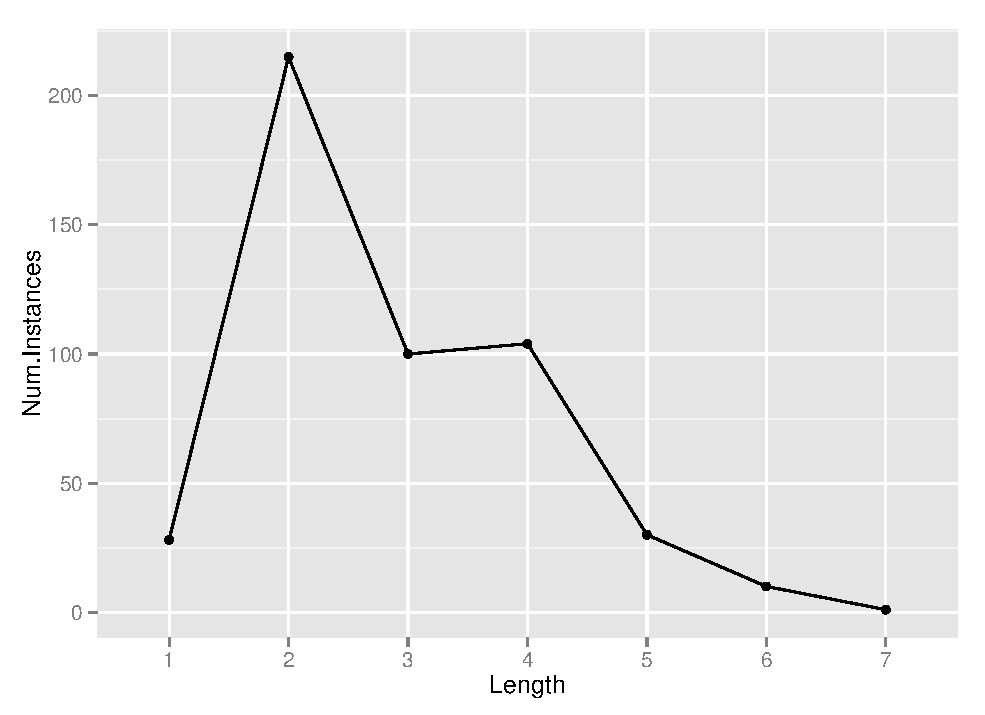
\includegraphics[scale=0.5]{Figures/length-numInstances-ibm-morph-sto.pdf}
    \caption{Number of instances by query length}
    \label{fig:morph-length-numInstances}
  \end{subfigure}
  \begin{subfigure}{0.49\textwidth}
    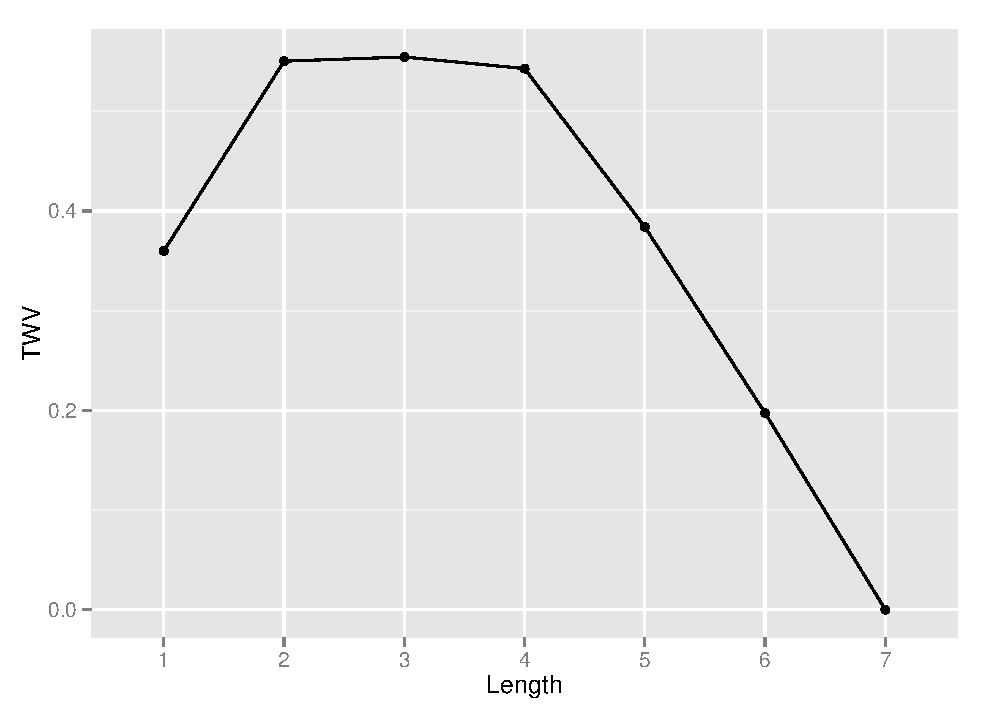
\includegraphics[scale=0.5]{Figures/length-twv-ibm-morph-sto.pdf}
    \caption{TWV by query length}
    \label{fig:morph-length-twv}
  \end{subfigure}
  \caption{Performance of IBM Morph STO system for various query lengths (i.e.\
  number of morphs in query)}
\end{figure}


\bibliographystyle{alpha}
\nocite{*}
\bibliography{refs}

\appendix

\section{Code Listings}

Our code is available at \path{/home/fl350/MLSALT5-practical/} on the MLSALT cluster.
In \autoref{sec:impl} we provide listings of our implementations and in
\autoref{sec:tests} we provide listings of our unit tests.

\subsection{Implementations}\label{sec:impl}~\\

\lstinputlisting[language=Scala,caption=An entry in KWS
index,label=lst:ctmEntry]{../src/main/scala/com/feynmanliang/kws/CTMEntry.scala}
\lstinputlisting[language=Scala,caption=Word-based KWS
system,label=lst:kwsIndex]{../src/main/scala/com/feynmanliang/kws/KWSIndex.scala}
\lstinputlisting[language=Scala,caption=Result of a KWS
query,label=lst:queryResult]{../src/main/scala/com/feynmanliang/kws/QueryResult.scala}

\lstinputlisting[language=Scala,caption=Performs morphological decomposition
using morph
dicts,label=lst:morphDecompose]{../src/main/scala/com/feynmanliang/kws/MorphDecompose.scala}
\lstinputlisting[language=Scala,caption=Morph-based KWS system which
automatically applies morph decomposition to the query as well as to index
entries if
required,label=lst:kwsIndexMorph]{../src/main/scala/com/feynmanliang/kws/KWSIndexMorph.scala}

\lstinputlisting[language=Scala,caption=Performs system combination by running
multiple KWS systems in parallel and unioning the
\texttt{QueryResults},label=lst:resultCombiner]{../src/main/scala/com/feynmanliang/kws/ResultCombiner.scala}

\lstinputlisting[language=Scala,caption=Generates a \texttt{map} file mapping
keyword IDs to their
lengths]{../src/main/scala/com/feynmanliang/kws/LengthMap.scala}

\subsection{Tests}\label{sec:tests}~\\

\lstinputlisting[language=Scala]{../src/test/scala/com/feynmanliang/kws/KWSIndexSpec.scala}

\lstinputlisting[language=Scala]{../src/test/scala/com/feynmanliang/kws/QueryResultSpec.scala}

\lstinputlisting[language=Scala]{../src/test/scala/com/feynmanliang/kws/MorphDecomposeSpec.scala}

\lstinputlisting[language=Scala]{../src/test/scala/com/feynmanliang/kws/KWSIndexMorphSpec.scala}

\end{document}

